\section{Theory}

	\subsection{Stuart-Landau-Oscillator}
	The Stuart-Landau oscillator is a dynamical system often used to model basic class 1 lasers.
	
	\begin{equation}	
		\dot{z}(t) = (\lambda +  i \omega + \gamma |z(t)|^2 ) z(t)
		\label{eq:stuartlandauequation}		
	\end{equation}

	\begin{figure}
		\centering
		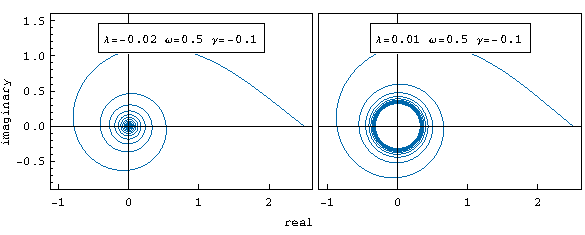
\includegraphics[width=0.99\linewidth]{pics/stuart_landau_complex_Focus_LC}
		\caption{$2$ very basic Stuart-Landau-scenarios: Decay towards a single fixed point (left) or towards a limit cycle (right).}
		\label{fig:stuart_spiral}
		%nicht mehr
		%stuart_landau_basic.nb
	\end{figure}

As can be seen in (eq. \ref{eq:stuartlandauequation}), the equation has a linear and a nonlinear term regarding the absolute value of $z$.

\subsection{Networks}

Vertices blabla \
Edges blabla. \

	\subsubsection{circulant Matrix}
    A circulant matrix has the same entries its row vectors, but with its entries rotated one element to the right relative to the previous row.
    
\subsection{virtual Nodes and multiplexing}
	here: papers for explanation!
	By multiplexing the input signal one can create virtual nodes in a network. The analogy to a real network can be best understood if the input signal is masked with a binary mask containing only values of either $0$ or $1$. 
	

\begin{figure}
	\centering
	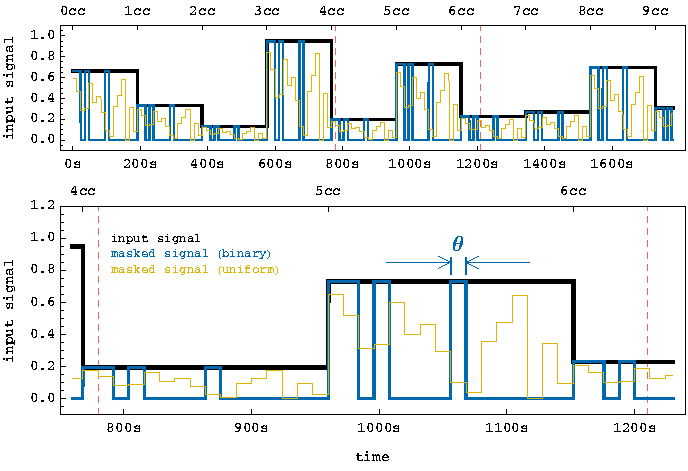
\includegraphics[width=0.99\linewidth]{pics/signal_mask_vis}
	\caption{A timeseries (black) with constant interpolation ("sample \& hold") between samples and the corresponding masked signal (blue). The mask length is counted in clockcycles (cc) and the time per virtual node is counted in $\theta$. Here $\theta = 12s$ and $1cc = 16 \theta = $}
	\label{fig:signal_mask_vis}
	%feedInVis_stuartlandau.nb
\end{figure}

	

\subsection{Dynamics of rings of stuart landau oscillators}
	pony-states (von André)
	
	

% different stuart landau scenarios - hopf bifurcation